\documentclass[border=1mm]{standalone}
%\documentclass[11pt]{article}
\usepackage{amsfonts,tikz,tikz-layers}
\usepackage{rotating,amsmath,amssymb}
\usetikzlibrary{fadings,quotes, shapes,calc,decorations.markings}
\usetikzlibrary{patterns}
\usetikzlibrary{shadows.blur}
\usetikzlibrary{shapes,shapes.geometric,positioning, arrows, arrows.meta}
\usetikzlibrary{backgrounds}

\def\MarkLt{6*1.7pt}
\def\MarkSep{3*1.7pt}
\tikzset{
  OneMark/.style={
    postaction={decorate,
      decoration={
        markings,
        mark=at position #1 with
          {
              \draw[-] (0,-\MarkLt) -- (0.5,\MarkLt) ;
          }
       }
    }
  },
  OneMark/.default={0.5}
}

\tikzset{
  OneMark2/.style={
    postaction={decorate,
      decoration={
        markings,
        mark=at position #1 with
          {
              \draw[-] (0,-\MarkLt) -- (-.5,\MarkLt) ;
          }
       }
    }
  },
  OneMark/.default={0.5}
}

\begin{document}
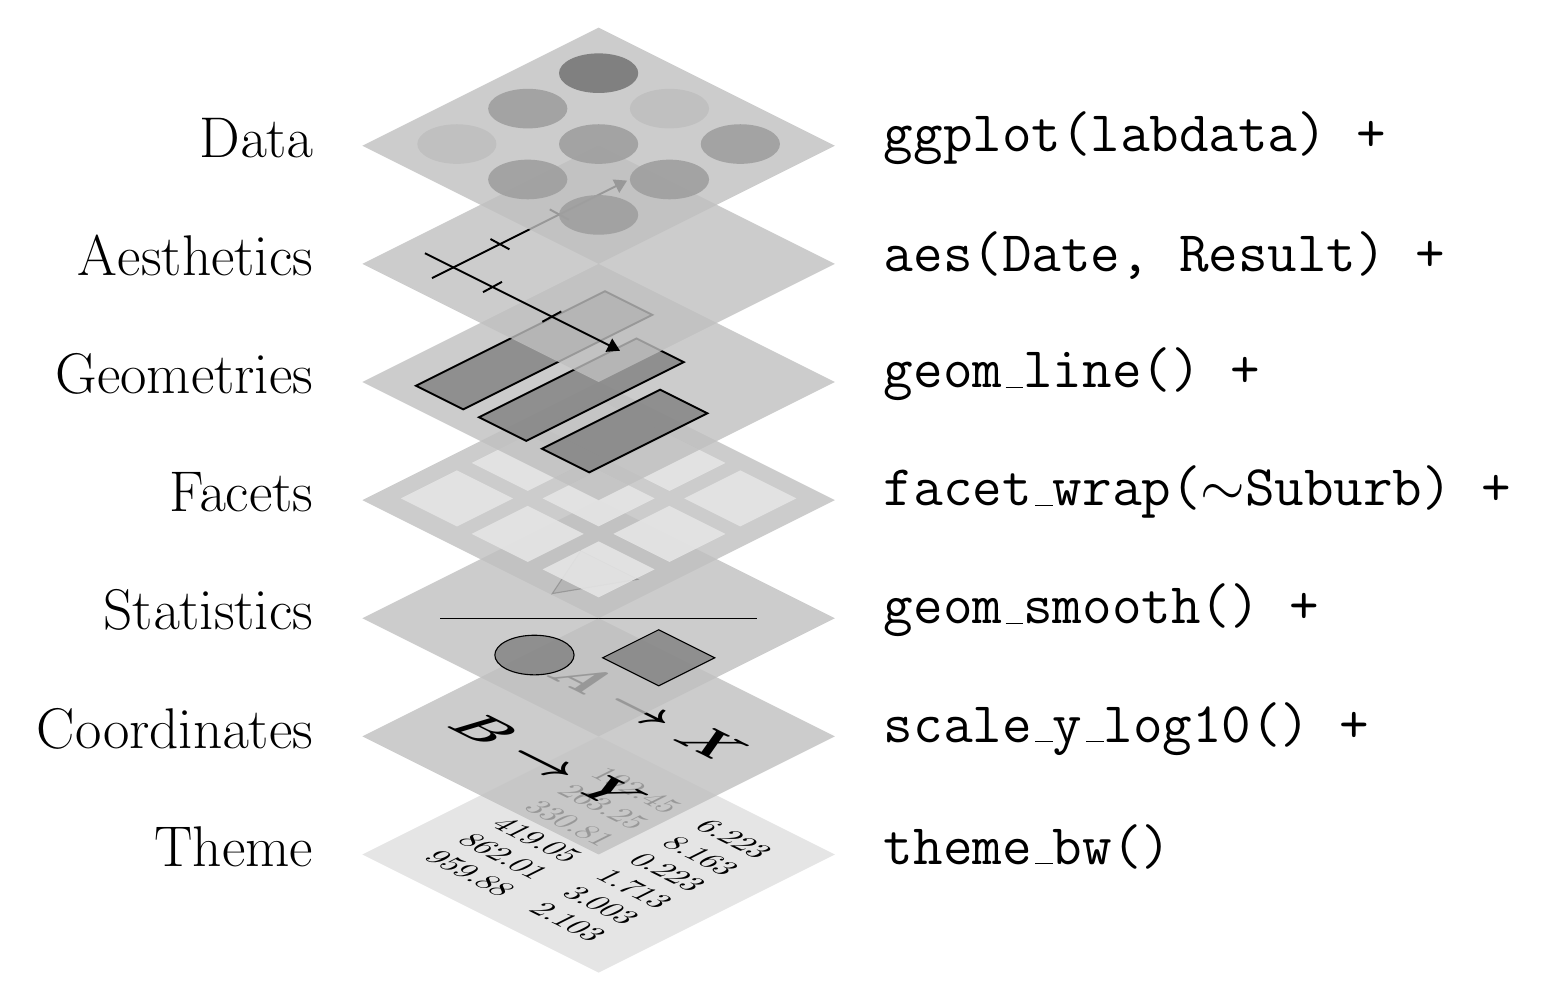
\begin{tikzpicture}[scale=.9,every node/.style={minimum size=1cm},on grid]
        \begin{scope}[  % Upper layer
            every node/.append style={
            yslant=0.5,xslant=-1},yslant=0.5,xslant=-1]

            %-----------------------------------------------
            \node[fill=lightgray,fill opacity=.4, minimum size=3cm,rotate=-90,shift={(1.5*6,-1.5*6)}] (G) {};
            \node[align=center,rotate=-90,font=\normalsize] at (G) {
            192.45$\quad$6.223\\
            263.25$\quad$8.163\\
            330.81$\quad$0.223\\
            419.05$\quad$1.713\\
            862.01$\quad$3.003\\
            959.88$\quad$2.103};
            %-----------------------------------------------
            \node[fill=lightgray,fill opacity=.8, minimum size=3cm,rotate=-90,shift={(1.5*5,-1.5*5)}] (F) {};
            \node[align=center,rotate=-90,font=\LARGE] at (F) {$\boldsymbol{A\rightarrow X}$\\[.5cm]$\boldsymbol{B\rightarrow Y}$};
            %-----------------------------------------------
            \node[fill=lightgray,fill opacity=.8, minimum size=3cm,rotate=-90,shift={(1.5*4,-1.5*4)}] (E) {};
            \draw[, shorten <=10mm, shorten >=10mm] (E.south west)--node[circle, draw,fill=gray,fill opacity=.8, scale=.25mm, below left=3mm,pos=.4] {} node[draw,fill=gray,fill opacity=.8, scale=.25mm, below left=2mm,pos=.65] {} node[rotate=90,scale=.25mm, above right=7mm,pos=.5] (tri) {} (E.north east);
            \draw[fill=gray,fill opacity=.8] (tri.north)--(tri.south west)--(tri.south east)--cycle;
            %---------------------------
            \node[fill=lightgray,fill opacity=.8, minimum size=3cm,rotate=-90,shift={(1.5*3,-1.5*3)}] (D) {};
            \node[fill=white!80!gray,fill opacity=.9, scale=.25mm] (c1) at ([xshift=-6.5mm, yshift=-6.5mm]D.north west) {};
            \foreach \i[count=\j from 2] /\k/\l in {1/brown/yshift,2/blue/yshift,1/red/xshift,4/yellow/yshift,5/teal/yshift,4/green/xshift,7/gray/yshift,8/orange/yshift}
            \node[fill=white!80!gray,fill opacity=.9, scale=.25mm] (c\j) at ([\l=-1cm]c\i) {};
             %--------------------------------------------
            \node[fill=lightgray,fill opacity=.8, minimum size=3cm,rotate=-90, shift={(1.5*2,-1.5*2)}] (C) {};
            \node[draw,fill=gray,fill opacity=.8, minimum width=2.4cm, minimum height=.6cm, anchor= south,line width=.7pt, xshift=1.5cm, yshift=.5cm] at (C.south) {};
            \node[draw,fill=gray,fill opacity=.8, minimum width=2cm, minimum height=.6cm, anchor= south,line width=.7pt, xshift=1.3cm, yshift=-.3cm] at (C.south) {};
            \node[draw,fill=gray,fill opacity=.8, minimum width=1.5cm, minimum height=.6cm, anchor= south,line width=.7pt, xshift=1.05cm, yshift=-1.1cm] at (C.south) {};
            %-----------------------------------------------
            \node[fill=lightgray,fill opacity=.8, minimum size=3cm,rotate=-90, shift={(1.5,-1.5)}] (B) {};
            \draw[-Triangle, shorten <=3mm, shorten >=3mm, line width=.7pt,OneMark=0.3, OneMark=0.55] ([xshift=.6cm]B.south west)--([xshift=.6cm]B.south east);
            \draw[-Triangle, shorten <=3mm, shorten >=3mm, line width=.7pt,OneMark2=0.45, OneMark2=0.7] ([yshift=-.7cm]B.south west)--([yshift=-.7cm]B.north west);
             %------------------------------------------------------
            \node[fill=lightgray,fill opacity=.8, minimum size=3cm,rotate=-90] (A) {};
            \node[circle, fill=gray, scale=.25mm] (c1) at ([xshift=-6.5mm, yshift=-6.5mm]A.north west) {};

            \foreach \i[count=\j from 2] /\k/\l in {1/gray/yshift,2/darkgray/yshift,1/darkgray/xshift,4/darkgray/yshift,5/darkgray/yshift,4/gray/xshift,7/darkgray/yshift,8/darkgray/yshift}
            \node[circle, fill=\k!50,fill opacity=.9, scale=.25mm] (c\j) at ([\l=-1cm]c\i) {};
        \end{scope}
        % Text
        \node[left=3.5cm of G, yshift=1mm,anchor=east] {\huge{Theme}};
        \node[left=3.5cm of F, yshift=1mm,anchor=east] {\huge{Coordinates}};
        \node[left=3.5cm of E, yshift=1mm,anchor=east] {\huge{Statistics}};
        \node[left=3.5cm of D, yshift=1mm,anchor=east] {\huge{Facets}};
        \node[left=3.5cm of C, yshift=1mm,anchor=east] {\huge{Geometries}};
        \node[left=3.5cm of B, yshift=1mm,anchor=east] {\huge{Aesthetics}};
        \node[left=3.5cm of A, yshift=1mm,anchor=east] {\huge{Data}};

        \node[right=3.5cm of A, yshift=1mm,anchor=west] {\huge{\texttt{ggplot(labdata) +}}};
        \node[right=3.5cm of B, yshift=1mm,anchor=west] {\huge{\texttt{aes(Date, Result) +}}};
        \node[right=3.5cm of C, yshift=1mm,anchor=west] {\huge{\texttt{geom\_line() +}}};
        \node[right=3.5cm of D, yshift=1mm,anchor=west] {\huge{\texttt{facet\_wrap($\sim$Suburb) +}}};
        \node[right=3.5cm of E, yshift=1mm,anchor=west] {\huge{\texttt{geom\_smooth() +}}};
        \node[right=3.5cm of F, yshift=1mm,anchor=west] {\huge{\texttt{scale\_y\_log10() +}}};
        \node[right=3.5cm of G, yshift=1mm,anchor=west] {\huge{\texttt{theme\_bw()}}};

\end{tikzpicture}


\end{document}
